\lecture[3]{3. Krappi og vindingur}{lecture-text}
\date{12.~janúar 2015}
\newcounter{mycount}
\refstepcounter{mycount}

\begin{document}

\begin{frame}
	\maketitle
\end{frame}




\begin{frame}{Einingarsnertivigur} 

\begin {block}{Skilgreining 3.\arabic{mycount}}\stepcounter{mycount}
Látum $\cal C$ vera feril í plani eða rúmi.
Látum $\rv$ vera stikun á $\cal C$ og gerum ráð fyrir að $\rv$ sé
þjáll stikaferill (þ.e.a.s.~$\rv$ er samfellt diffranlegur stikaferill og
$\rv'(t)\neq \ov$ fyrir öll $t$).  {\em Einingarsnertivigurinn} $\Tv$ við
ferilinn $\cal C$ í punktinum $\rv(t)$ er skilgreindur  með formúlunni  
$$\Tv=\frac{\rv'(t)}{|\rv'(t)|}=\frac{\vv(t)}{|\vv(t)|}.$$
\end{block}

\end{frame}

\begin {frame}{Krappi}
 \begin {block}{Skilgreining 3.\arabic{mycount}}\stepcounter{mycount}
   Látum $\cal C$ vera feril í plani eða rúmi og
$\rv$ stikun á $\cal C$ með bogalengd.  (Þegar fjallað er um stikanir
með bogalengd er venja að tákna stikann með $s$.) Lengd hraðavigurs
 er alltaf 1 og
því er $\Tv(s)=\vv(s)$.   {\em Krappi} (e.~curvature) ferilsins $\cal
C$ í punktinum $\rv(s)$ er skilgreindur sem talan 
$$\kappa(s)=\left|\frac{d\Tv}{ds}\right|.$$
{\em Krappageisli} (e.~radius of curvature) í punktinum $\rv(s)$ er
skilgreindur sem  
$$\rho(s)=\frac{1}{\kappa(s)}.$$
 \end {block}

\end {frame}

\begin {frame}{Meginþverill}
 \begin {block}{Skilgreining 3.\arabic{mycount}}\stepcounter{mycount}
   Látum $\cal C$ vera feril í plani eða rúmi og $\rv$ stikun á $\cal C$ með bogalengd.  {\em Meginþverill} (e.~unit principal normal) í punkti $\rv(s)$ er skilgreindur sem vigurinn 
$$\Nv(s)=\frac{\Tv'(s)}{|\Tv'(s)|}=\frac{1}{\kappa(s)}\Tv'(s).$$
 \end {block}

\end {frame}

\begin {frame}
 \begin {block}{Umræða 3.\arabic{mycount}}\stepcounter{mycount}
  Táknum með $\theta$ hornið sem $\Tv$ myndar við grunnvigurinn $\iv$. Þá er $\kappa = \frac{d\theta}{ds}$.
 \end {block}
 \begin{figure} [h]
\begin {center} \scalebox{0.65 }{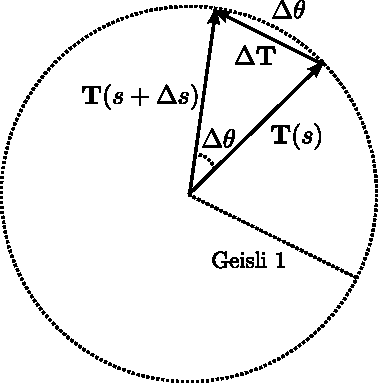
\includegraphics{krappi}} \end {center}
\end {figure}      
\end {frame}


\begin {frame}{Hjúfurplan}
 \begin {block}{Skilgreining 3.\arabic{mycount}}\stepcounter{mycount}
   Látum $\cal C$ vera feril í plani eða rúmi og $\rv$ stikun á $\cal C$ með bogalengd.  

{\em Hjúfurplanið} (e.~osculating plane) við ferilinn í punkti $\rv(s)$ er planið sem spannað er af  vigrunum $\Tv(s)$ og $\Nv(s)$ og liggur um punktinn $\rv(s)$.

{\em Hjúfurhringur} (e.~osculating circle) við ferilinn í punkti
$\rv(s)$ er hringur sem liggur í hjúfurplaninu, fer í gegnum punktinn
$\rv(s)$, hefur geisla $\rho(s)$ og hefur miðju í punktinum
$\rv(s)+\rho(s)\Nv(s)$. 
 \end {block}

\end {frame}

\begin {frame}{Tvíþverill}
 \begin {block}{Skilgreining 3.\arabic{mycount}}\stepcounter{mycount}
   Látum $\cal C$ vera feril í plani eða rúmi og
$\rv$ stikun á $\cal C$ með bogalengd.  Vigurinn  
$$\Bv(s)=\Tv(s)\times \Nv(s)$$
kallas {\em tvíþverill} (e.~binormal) við ferilinn í $\rv(s)$.
 \end {block}

 \bigskip
 $\{\Tv(s),\Nv(s),\Bv(s)\}$ er þverstaðlaður grunnur og kallast \textbf{Frenet ramminn}.
\end {frame}

\begin {frame}{Vindingur}
 \begin {block}{Setning og skilgreining 3.\arabic{mycount}}\stepcounter{mycount}
  Látum $\cal C$ vera feril í plani
eða rúmi og $\rv$ stikun á $\cal C$ með bogalengd.  Vigurinn $\Bv'(s)$ er
samsíða vigrinum $\Nv(s)$, þ.e.a.s.~$\Bv'(s)$ er margfeldi af $\Nv(s)$.
Talan $\tau(s)$ þannig að  
$$\Bv'(s)=-\tau(s)\Nv(s)$$
kallast {\em vindingur} ferilsins í punktinum $\rv(s)$.

 \end {block}

\end {frame}


\begin {frame}{Frenet-Serret jöfnurnar}
 \begin{block}{Jöfnur 3.\arabic{mycount}}\stepcounter{mycount}
   Látum $\cal C$ vera feril í plani
eða rúmi og $\rv$ stikun á $\cal C$ með bogalengd.  Þá gildir 
\begin{align*}
\Tv'(s)&=\kappa\Nv\\
\Nv'(s)&=-\kappa\Tv+\tau\Bv\\
\Bv'(s)&=-\tau\Nv.
\end{align*}
 \end{block}

\end {frame}

\begin {frame}
 \begin {block}{Setning 3.\arabic{mycount}}\stepcounter{mycount}
   Látum $\cal C$ vera feril í plani eða rúmi. 
Gerum ráð fyrir að $\rv$ sé þjáll stikaferill
sem stikar $\cal C$. Ritum $\vv=\rv'(t)$ og $\av=\rv''(t)$.
Þá gildir í punktinum $\rv(t)$ að
$$\Tv=\frac{\vv}{|\vv|},\qquad 
\Bv=\frac{\vv\times\av}{|\vv\times\av|},\qquad
\Nv=\Bv\times\Tv,$$
einnig er 
$$\kappa=\frac{|\vv\times\av|}{|\vv|^3},\qquad\qquad
\tau=\frac{(\vv\times\av)\cdot \frac{d}{dt}\av}{|\vv\times\av|^2}.$$

 \end {block}

\end {frame}

\end{document}